\chapter[\softwarename{minspec}]{\softwarename{minspec}, a bioinformatic tool for metagenomics}
\label{ch:minspec}

\previouslypublished{Sections of this chapter have been previously published in \bibentry{Wilkins:2012wg}.}

\section{Summary}

\section{Introduction}

\subsection{Metagenomic analysis of microbial assemblages}

The identification of the species or \acp{OTU} that compose a microbial community is a primary aim of metagenomics.
Typically this is achieved using one of two methods.

The first method is the identification, using a search and alignment algorithm such as \softwarename{blast}, of specific marker genes or other sequences which are diagnostic for a particular \ac{OTU}.
Common targets in microbial ecology are the 16S or other ribosomal subunit rDNA sequences, and the \ac{ITS} regions between 16S--23S rDNA sequences \citep[e.g.][]{Brown:2012gna}.
This method provides several advantages.
The selected regions are usually highly conserved, and through cultivation and full-genome sequencing have been reliably associated with a particular \ac{OTU}, allowing very accurate identification and analysis of diversity down to the ecotype level \citep[e.g.][]{Brown:2012gna}.
If the copy number of the gene or region is well known, this method also allows for accurate estimations of cell abundance from metagenomes.
However, a disadvantage of this method is that the large majority of metagenomic reads which do not happen to cover the region of interest will contribute nothing to the analysis and essentially be wasted.
Low-abundance \acp{OTU} will therefore be missed, as even if they generate a small number of reads, those reads are unlikely to cover the region of interest.

The second method is to compare assembled or unassembled metagenomic reads to a reference database, using an algorithm such as \softwarename{blast}, then use probabilistic methods to assign identifications and abundances with varying degrees of confidence.
Most commonly, the reads are compared to a database of full genomes \citep[e.g.][]{Lauro:2010jna,Qin:2010fl}.
This method makes more efficient use of metagenomic data compared to the first, as any read can potentially yield a \softwarename{blast} match and thus contribute to the identification of an \ac{OTU}.
However, interpretation of the results, and particularly calculation of abundances, is more complex.
For example, the software tool \ac{GAAS} makes use of \softwarename{blast} match quality, number of matches and estimated genome size to estimate the relative abundances of \acp{OTU} in a sample \cite{Angly:2009ip}.

Such estimates are confounded by the presence of multiple \acp{OTU} which can generate high-quality \softwarename{blast} matches (``hits'') to a given read.
Multiple high-quality hits to a single read are the norm, rather than the exception, in metagenomic studies for several reasons.
A microbial assemblage will often include a number of closely-related \acp{OTU} (e.g.\ congeners) which share large sections of highly similar or identical genomic sequence.
If several such \acp{OTU} are present in the reference database, a metagenomic read from one will yield high-quality \softwarename{blast} hits to them all.
Further, even distantly related \acp{OTU} are likely to share large regions of identity, and the selection of hit quality thresholds to discriminate between them (for example, a minimum bit score or maximum expectation value) is effectively arbitrary.
Thus, while metagenomic studies using whole-genome comparisons almost always use such thresholds as the sole discriminators between \acp{OTU}, this method (hereafter the ``\naive'' method, after \citet{Ye:2009bl}) will almost inevitably result in the identification of \acp{OTU} which are not present in the assemblage, skewing the relative abundance estimates of those which are truly present.

\begin{table}
\small
\caption[Examples of spurious species identifications]{Selected examples of species identified in a marine metagenome using \naive identification.
These species were identified in a single sample from the \ac{SO} (sample 346; see \ref{chp:polarfront}).
The sample was compared to the RefSeq database of full genomes using \softwarename{tblastx} with an E-value maximum of $1.0\times{}10^{-3}$, i.e.\ only high-quality hits were included.
Relative abundances were calculated using \softwarename{GAAS} \cite{Angly:2009ip}.
}
\label{tab:unlikelyotus}
\smallskip
\begin{tabularx}{\textwidth}{XlX}
\toprule
\textbf{Species} & \textbf{Relative} & \textbf{Notes}\\
& \textbf{Abundance (\%)}&\\
\midrule
Encephalomyocarditis virus & 1.98 & Human pathogen.\\
Marek's disease virus type 1 & 1.49 & Chicken pathogen.\\
Marek's disease virus type 2	& 0.85 & Chicken pathogen.\\
\speciesfull{Francisella philomiragia}& 0.041 & Human and animal pathogen.\\
\speciesfull{Agrobacterium vitis} & 0.040 & Plant and opportunistic human pathogen.\\
\speciesfull{Brucella suis} & 0.011 & Human and swine pathogen (causes brucellosis).\\
\genus{Enterobacter} sp. 638	& 0.0085 & Animal commensal/pathogen.\\
\speciesfull{Bordetella parapertussis} & 0.0075 & Mammalian pathogen (causes mild form of whooping cough).\\
\speciesfull{Neisseria meningitidis} & 0.0074 & Human pathogen.\\
\speciesfull{Yersinia pestis} & 0.0060 & Human/animal pathogen (causes bubonic plague).\\
\bottomrule
\end{tabularx}
\end{table}


This problem is compounded by a systematic overrepresentation within databases of reference genomes of taxa of interest to humans, such as human and agricultural pathogens.
Environmental \acp{OTU} are comparatively underrepresented.
For example, \tabreft{tab:unlikelyotus} gives examples of terrestrial plant and animal pathogens, \textit{a priori} unlikely to be truly present, which were identified in an open ocean metagenome using the \naive{} method.

One commonly used software tool to address this problem, \ac{MEGAN}, aggregates reads with hits to many \acp{OTU} to the most recent common ancestor of those \acp{OTU}, represented by a higher taxonomic rank e.g.\ family \cite{Huson:2007jl}.
This approach increases the fidelity of the results, but comes at the cost of reduced taxonomic resolution.
Particularly in marine assemblages where even fine genomic differences can represent distinct ecological functions \citep[e.g.][]{Brown:2012gna}, a tool which reduces spurious identifications without compromising taxonomic resolution would clearly be valuable. 

\subsection{The maximum parsimony approach}

\citet{Ye:2009bl} identified an analogous problem in the annotation of biochemical pathways in genomes and metagenomes.
They noted that a common method is to annotate a pathway as present if a single protein within that pathway attracts at least one high-quality \softwarename{blast} hit.
However, because many proteins are shared by multiple pathways, and databases of orthologous genes are often incomplete, this method has resulted in many clearly spurious annotations, such as an ascorbic acid synthesis pathway in the human genome (humans require dietary vitamin C) and a mitochondrial pathway in \species{Escherichia coli} (annotated in the \ac{KEGG} PATHWAY database).

The authors developed a software tool, \softwarename{MinPath}, to combat this problem and increase the accuracy and fidelity of pathway annotations.
\softwarename{MinPath} computes the smallest possible set of pathways (``maximum parsimony'') sufficient to explain a set of annotated proteins.
As a simple example, if a genome is annotated with all the proteins that belong to pathway A, and one of those proteins also happens to belong to pathway B --- that is, it is shared by both pathways --- the \naive{} approach would annotate both pathways as present.
However, the most parsimonious explanation is that pathway A is present, and B is not.

\softwarename{MinPath} was implemented by framing the construction of a maximum parsimony pathway set as an \ac{IP} problem.
\ac{IP} is a subset of algorithms for solving \ac{LP} problems, which seek to maximise the value of a linear function (the objective function) within a set of constraints.
In this case, the objective function was maximised by decreasing the number of annotated biochemical pathways, while the constraint was that every high-quality protein annotation had to be represented at least once in the annotated pathways.
Validation and testing of \softwarename{MinPath} showed it was successful in eliminating spuriously annotated pathways while retaining those genuinely present.

It was noted that this as this problem is essential isomorphic with that of spurious annotations in microbial metagenomes, the ``maximum parsimony'' method would likely also work in this domain.
The aim of the project described in this chapter was thus to develop and test a software tool, \softwarename{minspec}, which would find the most parsimonious set of \acp{OTU} necessary to explain a set of observed \softwarename{blast} hits generated by a metagenome, using the approach of \cite{Ye:2009bl} as a model.

\section{Methods}

\subsection{Implementation of \softwarename{minspec}}

A computational method to minimise false \ac{OTU} identifications and increase the accuracy of \ac{OTU} abundance estimates (\softwarename{minspec}) was developed and implemented in \softwarename{perl}\footnote{\softwarename{minspec} and the associated metagenomic simulation and validation scripts are open source and available at \url{https://github.com/wilkox/minspec}.}.
Following the approach of \citet{Ye:2009bl} to the parsimonious reconstruction of biochemical pathways (\softwarename{MinPath}), \softwarename{minspec} computes the smallest set of \acp{OTU} sufficient to explain a set of observed high-quality hits against RefSeq (or any other sequence database).
The minimal set computation was framed as a \ac{IP} problem and solved with \softwarename{glpsol} (The GNU Linear Programming/MIP solver) (Free Software Foundation, Boston).

The objective function for the \ac{IP} problem was constructed as follows \citep[adapted from][]{Ye:2009bl}:
\begin{equation*}
\mathrm{min}\sum_{j=1}^{s}A_{j}
\end{equation*}
where \textit{s} is the number of \acp{OTU} in the assemblage, and $A_{j} = 1$ if \ac{OTU} \textit{j} is in the assemblage, 0 if not.
In other words, the objective function is satisfied by minimising the number of \acp{OTU} in the assemblage.
The constraint function was constructed as follows \citep[adapted from][]{Ye:2009bl}:
\begin{equation*}
\sum_{j=1}^{s}M_{ij}A_{j}\ge1 \; \; \; \forall i \in [1,n]
\end{equation*}
where $M_{ij} = 1$ if read \textit{i} has a mapping (i.e.\ a high-quality \softwarename{blast} hit) to \ac{OTU} \textit{j}, 0 if not, and $[1,n]$ is the set of all reads.
In other words, the constraint function fails if any read does not have at least one of its high-quality \softwarename{blast} hits represented in the assemblage.

This approach eliminates many of the spurious \ac{OTU} identifications which result from reads with strong identity to more than one \ac{OTU}.
The ``minimal \ac{OTU} set'' is liable to exclude some low-abundance \acp{OTU}, but gives more faithful abundance estimates and eliminates many false positives.

It was noted that in some special cases, it may be desirable to include an \ac{OTU} in the assemblage even if it is not part of the minimal set, if that \ac{OTU} generated a very large number of \softwarename{blast} hits.
An example of such a situation might be if the sample was known with certainty to contain a two very closely related \acp{OTU} at roughly equal abundance.
In such a case, it would be expected that almost all metagenomic reads generated by each of these \acp{OTU} would also attract \softwarename{blast} hits to the other, and \softwarename{minspec} would thus probably eliminate whichever happened to generate slightly fewer hits.
To allow for this, an option was added such that \softwarename{minspec} will not eliminate \acp{OTU} to which a specified threshold number of reads attract high-quality hits.

\subsection{Validation of \softwarename{minspec}}

To establish the usefulness of \softwarename{minspec}, a validation method was devised to experimentally determine its error rates and efficacy (i.e.\ number of spurious \acp{OTU} identified and removed).

A set of simulated microbial \acp{OTU} was generated.
To simulate genomic sequence identity between \acp{OTU}, each simulated \ac{OTU} went through up to fifty rounds in which another \ac{OTU} was selected at random and marked as having sequence identity with the first.
This process was terminated with a 10\% probability at each round, simulating an exponential curve of interrelatedness between \acp{OTU}.
A random subset of the simulated \acp{OTU} were then selected to form a simulated microbial assemblage.
Because of the previously established simulated sequence identity between \acp{OTU}, some \acp{OTU} in the assemblage would be marked as having identity to other \acp{OTU} both within the assemblage and outside of it.

A simulated metagenomic sampling was then performed.
In each round, an \ac{OTU} was selected at random.
To produce a natural rank-abundance curve of \ac{OTU} abundance within the assemblage, the probability that the selected \ac{OTU} yielded a read was
\begin{equation*}
\frac{1}{ln(x)+1}
\end{equation*}
where $x$ is the \ac{OTU}'s rank.
Simulated \softwarename{blast} matches to the \ac{OTU} were generated for the read.
These matches would include accurate high-quality ``genuine'' hits to the \ac{OTU} that produced the read, as well as to other randomly selected \acp{OTU} both within and out of the assemblage which had been previously marked as having sequence identity to the ``genuine'' \ac{OTU}.

To fully explore the limits and reliability of \softwarename{minspec}, the simulated metagenomic experiment described above was performed with all possible permutations of the following parameters: number of simulated \acp{OTU} [100; 1,000; 10,000; 50,000; 100,000]; size of simulated assemblage [1; 10; 100; 300; 500; 1,000; 10,000]; number of simulated metagenomic reads [10; 100; 1,000; 10,000; 100,000; 200,000; 500,000].
Each permutation was repeated five times, except for those where the size of the assemblage would exceed the number of \acp{OTU} simulated.

The resulting simulated \softwarename{blast} outputs were processed with \softwarename{minspec}, and the false positive (percentage of \acp{OTU} not in the assemblage which nevertheless survived \softwarename{minspec} filtering) and false negative (percentage of \acp{OTU} present in the assemblage which were not present after \softwarename{minspec} filtering) rates calculated.
Because a high false negative rate can arise from undersampling, a problem in metagenomic studies both real and simulated, an additional ``false negative (\softwarename{minspec})'' metric was calculated, which excluded \acp{OTU} which were present in the assemblage but through random chance did not generate any reads, the equivalent of ``unsampled rare taxa''.
This rate thus represented only false negatives attributable to \softwarename{minspec} itself.
Finally, as a measure of \softwarename{minspec}'s usefulness, the proportion of ``false \acp{OTU}'' --- \acp{OTU} that generated \softwarename{blast} matches but were not part of the assemblage --- successfully removed by \softwarename{minspec} was calculated.

\section{Results}

Repeated simulated metagenomic experiments with a wide range of permutations of parameters showed that \softwarename{minspec} was reliable and able to substantially reduce the rate of false positive \ac{OTU} identifications, although its effectiveness varied with the parameters of the assemblage and metagenomic experiment \figref{fig:minspecvalidation}.

\begin{figure}
\begin{tabular}{cc}
\subfloat[\sffamily{}False negative rate (\%) --- the percentage of \acp{OTU} in the assemblage that were absent from the \softwarename{blast} results following \softwarename{minspec} processing.\label{fig:minspecvalidationfalsenegative}]{
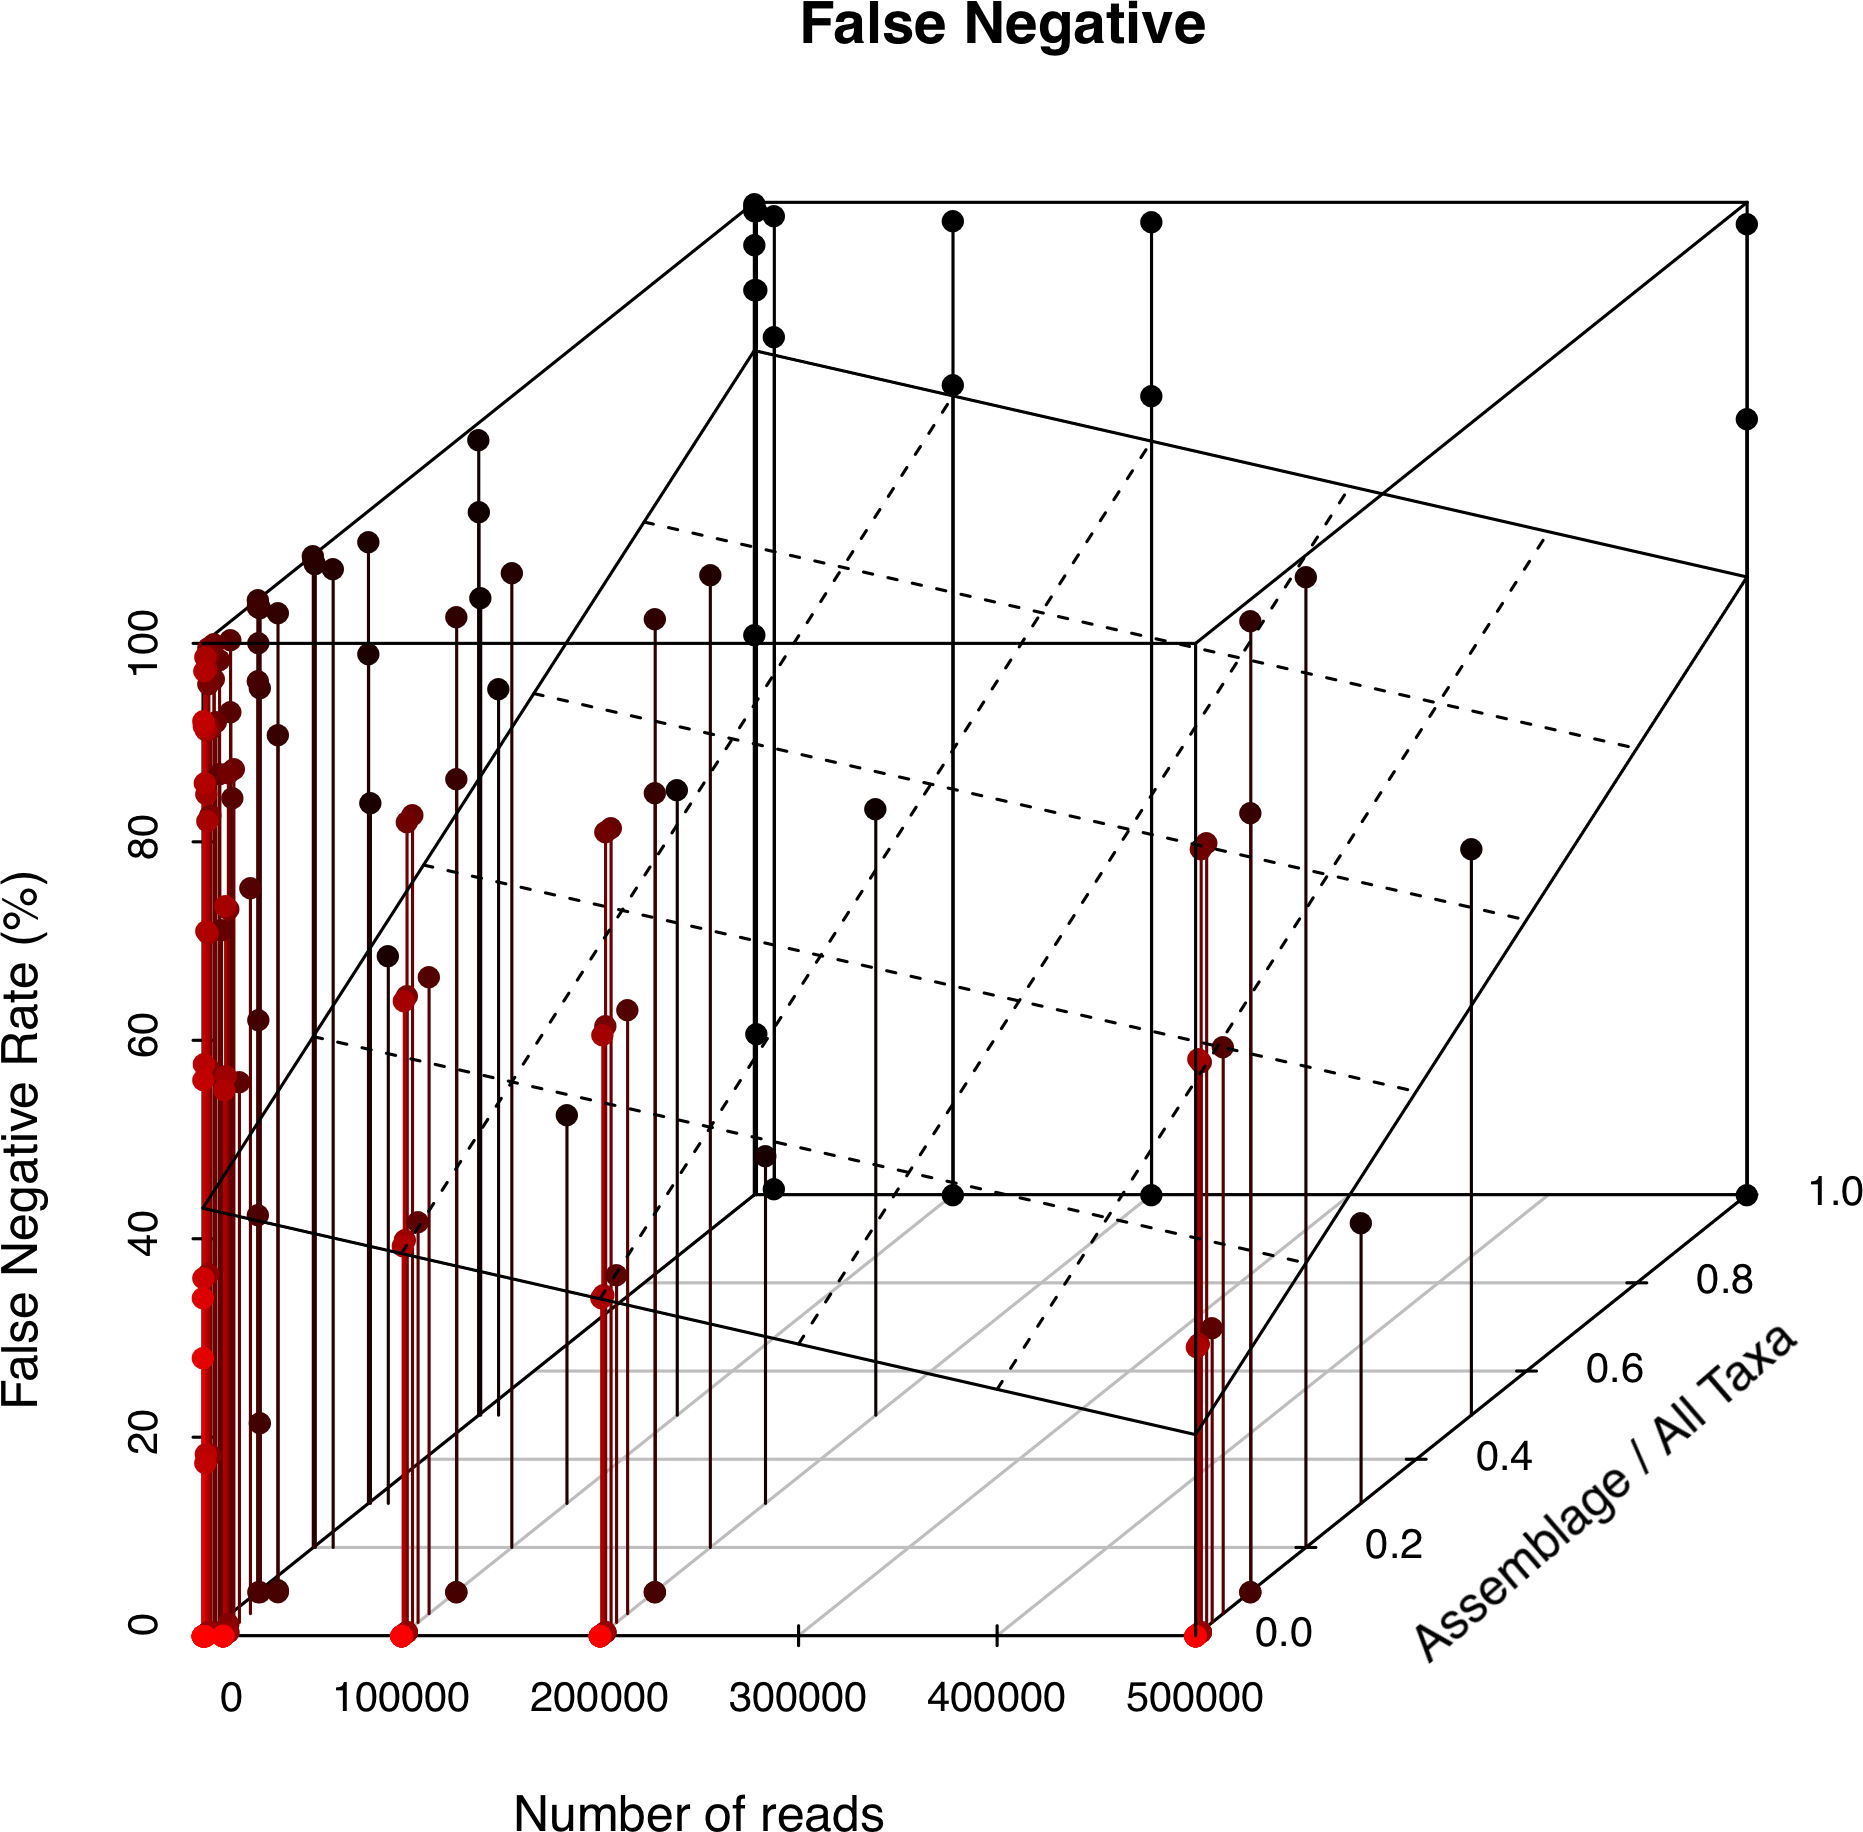
\includegraphics[width=0.45\textwidth]{../minspec/falsenegative.png}
}

&
%\quad %add desired spacing between images, e. g. ~, \quad, \qquad etc. 
%(or a blank line to force the subfigure onto a new line)

\subfloat[\sffamily{}\softwarename{minspec}-attributable false negative rate (\%) --- the percentage of \acp{OTU} not in the assemblage that generated \softwarename{blast} hits but were incorrectly removed by \softwarename{minspec}.\label{fig:minspecvalidationminspecfalsenegative}]{
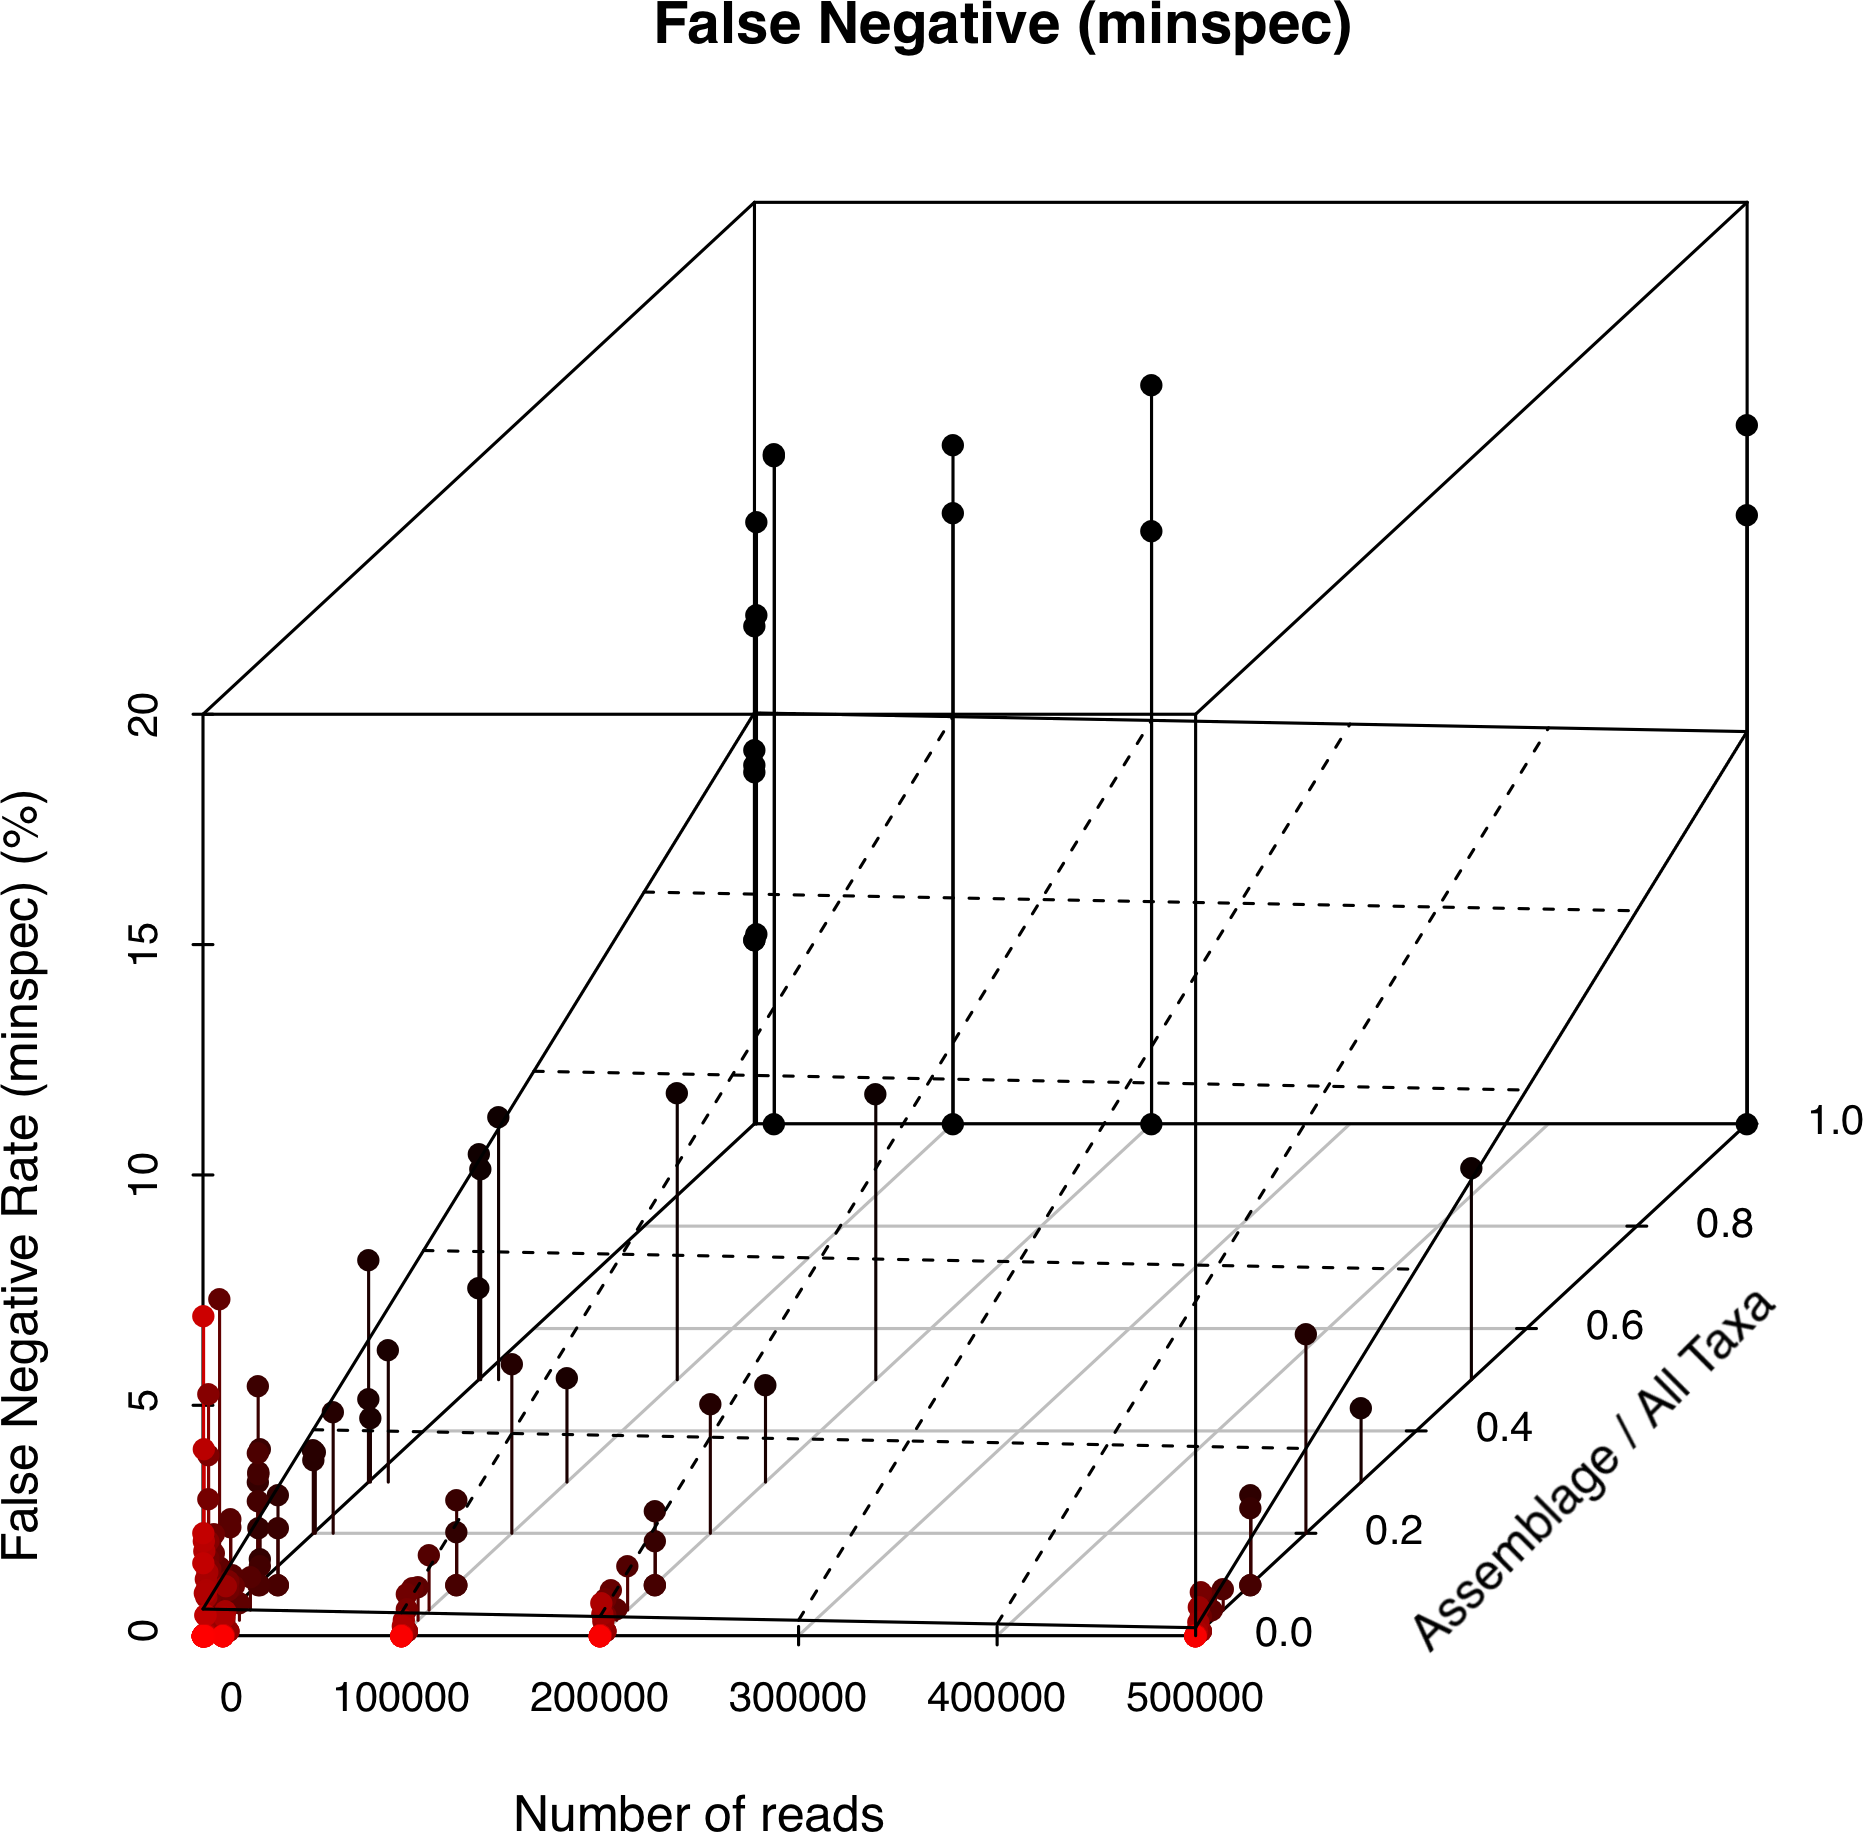
\includegraphics[width=0.45\textwidth]{../minspec/minspecfalsenegative.png}
}
\bigskip
\\
\bigskip
\\
%\quad %add desired spacing between images, e. g. ~, \quad, \qquad etc. 
%(or a blank line to force the subfigure onto a new line)

\subfloat[\sffamily{}False positive rate (\%) --- the percentage of \acp{OTU} not in the assemblage that were present in the \softwarename{blast} results following \softwarename{minspec} processing. \label{fig:minspecvalidationfalsepositive}]{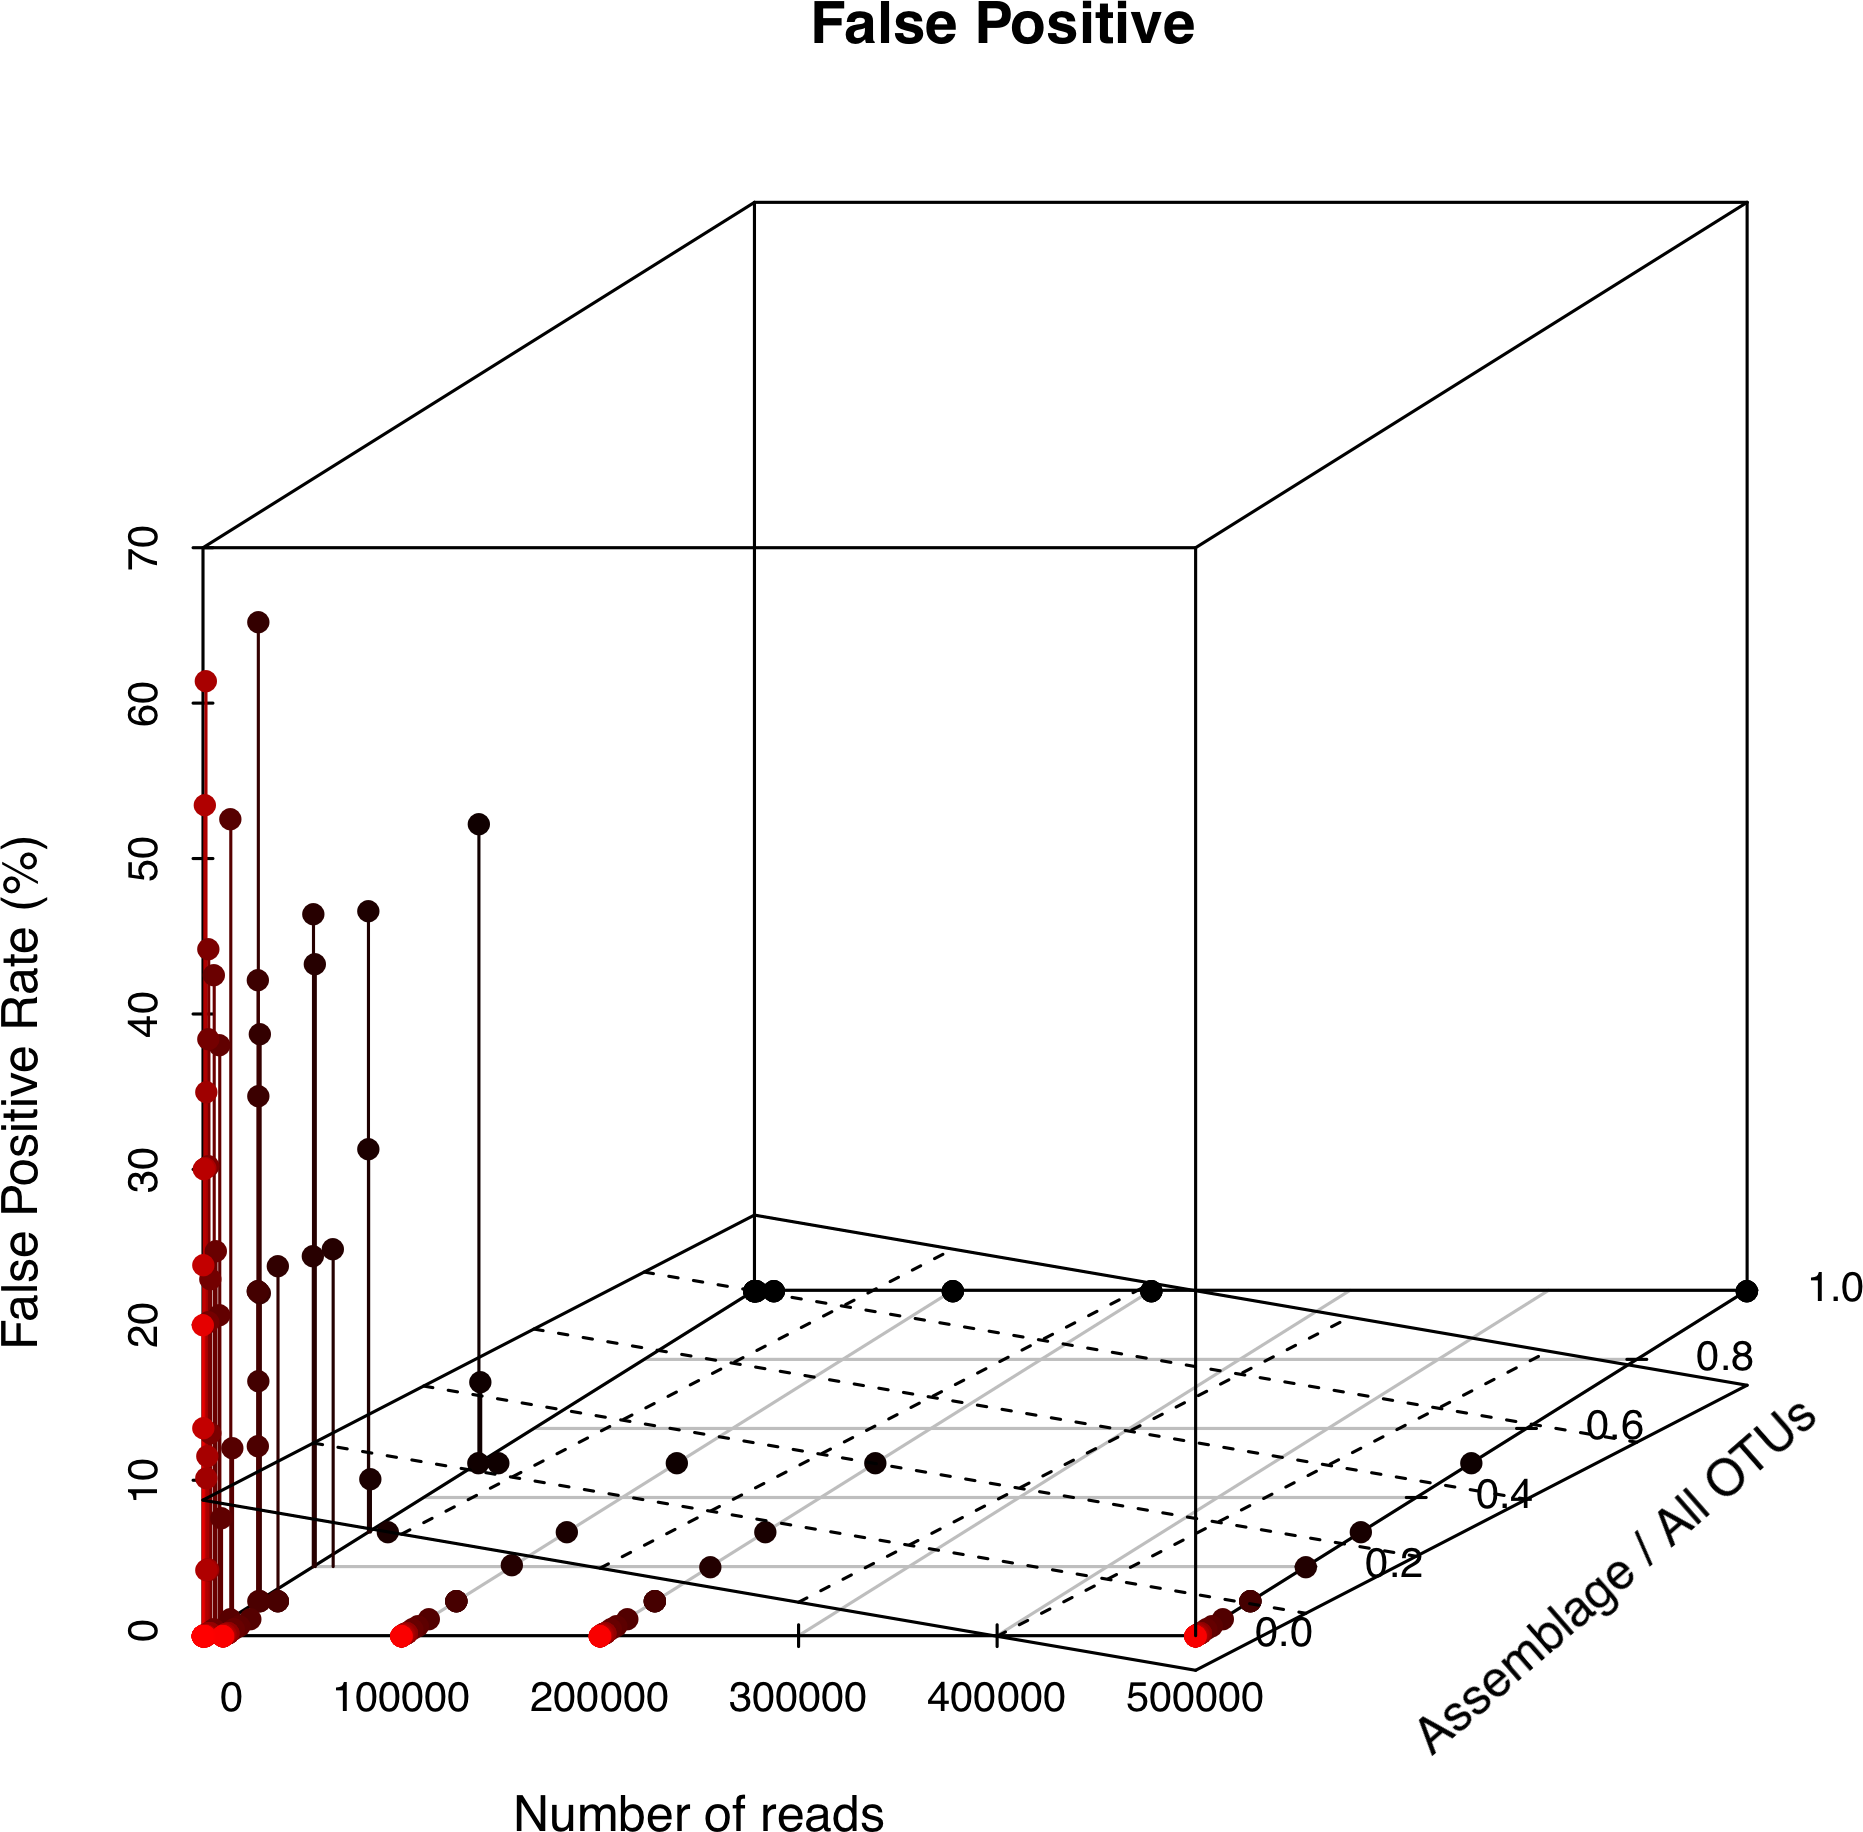
\includegraphics[width=0.45\textwidth]{../minspec/falsepositive.png}}

&
%\quad %add desired spacing between images, e. g. ~, \quad, \qquad etc. 
%(or a blank line to force the subfigure onto a new line)

\subfloat[\sffamily{}Proportion of false \acp{OTU} --- \acp{OTU} that were not part of the simulated assemblage but which generated hits due to simulated sequence identity --- that were correctly identified and removed by \softwarename{minspec}.\label{fig:minspecvalidationfalseotusaremoved}]{
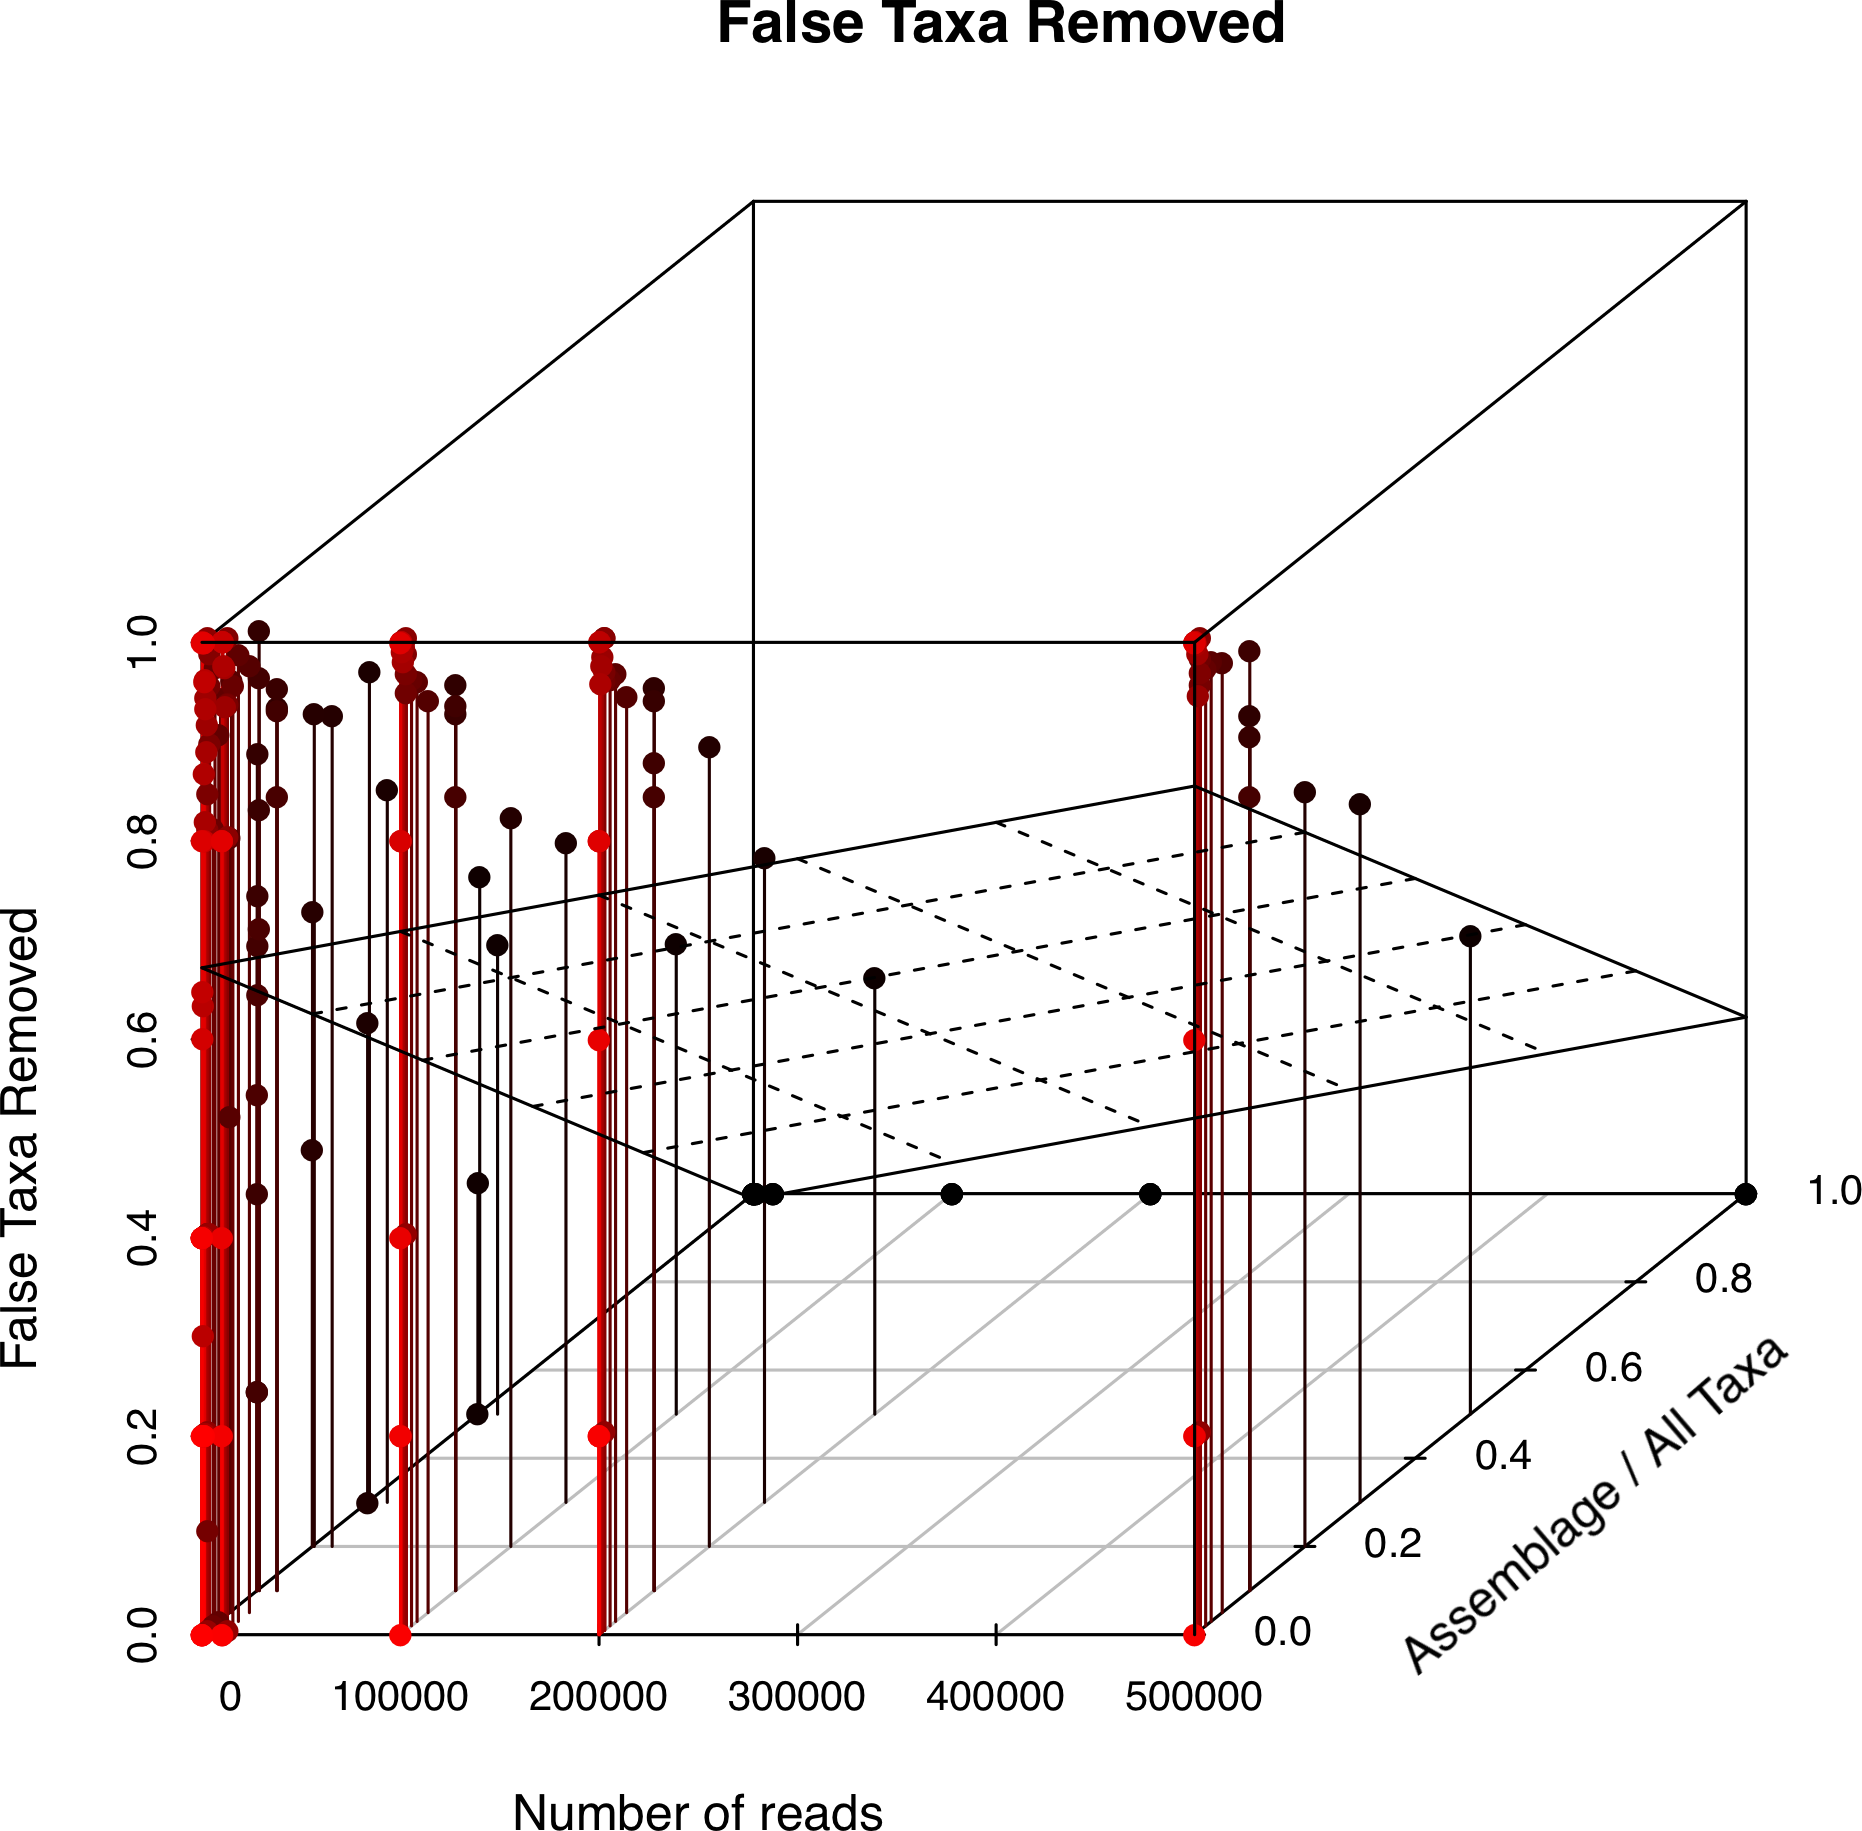
\includegraphics[width=0.45\textwidth]{../minspec/falseotusremoved.png}
}
\\

\end{tabular}

\caption[Results of \softwarename{minspec} validation]{Results of repeated trials of \softwarename{minspec} on simulated metagenomic studies with multiple permutations of parameters (number of reads, number of simulated \acp{OTU}, size of simulated assemblage).
The number of simulated \acp{OTU} and size of simulated assemblage are represented as a ratio on the z-axis (``assemblage / all \acp{OTU}'').
Each permutation was repeated five times.
A plane representing a linear regression has been overlaid on each plot to indicate the trend.
Points have been tinted to aid the perception of depth; colour is not otherwise meaningful.
}\label{fig:minspecvalidation}
\end{figure}


\section{Discussion}

The false negative rate, or percentage of \acp{OTU} in the simulated assemblage which were absent from the \softwarename{blast} results following \softwarename{minspec} processing, was generally high, ranging from \textapprox{}20\% under ideal conditions (a low assemblage / all \acp{OTU} ratio, and 500,000-read metagenomic sample) to \textapprox{}90\% in the worst case (a high assemblage / all \acp{OTU} ratio and a small metagenomic sample) \figref{fig:minspecvalidationfalsenegative}.
The assemblage / all \acp{OTU} ratio (hereafter referred to as ``assemblage ratio'') indicates the proportion of simulated \acp{OTU} (``all \acp{OTU}'') that were chosen to form the simulated assemblage.
A higher ratio means that any \ac{OTU} is more likely on average to be part of the assemblage, and thus that any individual failure to detect a \ac{OTU} is an error.
This problem is mitigated with increasing the number of reads, as this makes it less likely that a given \ac{OTU} would go unsampled.
The extreme false negative rates, in some cases 100\%, represent extreme simulated scenarios (e.g.\ an assemblage of 1 \ac{OTU} drawn from a pool of 100,000), and thus do not reflect real metagenomic studies.

Because the majority of false negatives are attributable to undersampling and failure of \acp{OTU} to generate \softwarename{blast} hits --- properties the simulated metagenomic experiments share with real ones --- a second metric, the false negative (\softwarename{minspec}) rate, was calculated \figref{fig:minspecvalidationminspecfalsenegative}.
This is the proportion of \acp{OTU} in the assemblage that generated \softwarename{blast} hits, but were incorrectly removed by \softwarename{minspec}.
This rate thus represents error attributable only to \softwarename{minspec}.
The false negative (\softwarename{minspec}) rate was generally low, ranging from \textapprox{}0--1\% for low assemblage ratios, to \textapprox{}15--20\% under high ratios.
Surprisingly, increasing the number of reads only slightly decreased the rate, at both low and high assemblage ratios.
This suggests \softwarename{minspec} is more affected by the degree of similarities between \acp{OTU} than by undersampling.

The false positive rate, or percentage of \acp{OTU} not in the assemblage which nevertheless generated high-quality \softwarename{blast} matches that were not identified and removed by \softwarename{minspec}, was generally \textapprox{}0--5\% except for extremely small read sets and low assemblage ratios, where it reached as high as 60\% \figref{fig:minspecvalidationfalsepositive}.
These results reinforce the value of larger read sets, and show that once a modest metagenome size is reached (\textapprox{}100,000 reads) very few false positives can be expected.

The proportion of false \acp{OTU} removed was calculated to measure \softwarename{minspec}'s efficacy in identifying and eliminating \ac{OTU} which are not part of the sampled assemblage yet generate high-quality \softwarename{blast} matches.
This rate varied from 0--1 depending on the parameters of the assemblage \figref{fig:minspecvalidationfalseotusremoved}.
For simulations with a low assemblage ratio, the proportion was generally high ($> 0.6$), although there were simulated experiments with a low ratio where the proportion was low or zero.
However, in all simulations with an assemblage ratio of 1, the proportion was 0, and the regression indicated a generally inverse relationship between the ratio and the proportion of false \acp{OTU} removed.
This is likely because in assemblages with a higher assemblage ratio, there are fewer false \acp{OTU} to remove; in assemblages with a ratio of 1, there are none.
The high proportion of false \acp{OTU} correctly identified in simulations with a low assemblage ratio is thus a good indication that \softwarename{minspec} is effective at identifying and removing false \acp{OTU}, especially as this proportion far exceeds the false positive and false negative (\softwarename{minspec}) rates for comparable experiments.
As expected, increasing the number of reads improved \softwarename{minspec}'s accuracy.

\section{Conclusions}

Overall, the simulated experiments validated both the accuracy and usefulness of \softwarename{minspec} as a tool for reducing error in metagenomic studies.
It is worth noting that the assemblage ratio is not an inherent property of an assemblage, although it is limited by the assemblage's \ac{OTU} richness.
Rather, it can be decreased, and thus the accuracy of the metagenomic experiment improved, by performing \softwarename{blast} searches against larger databases with finer taxonomic resolution.
These results thus reinforce the value of both large read sets and comprehensive reference databases in obtaining high-quality metagenomic results.

At the time of writing, \softwarename{minspec} has been used in two published projects: \citet{Wilkins:2012wg} and \citet{Williams:2012gsa}.
